%!TEX program = xelatex

\documentclass[compress]{beamer}
%--------------------------------------------------------------------------
% Common packages
%--------------------------------------------------------------------------
\usepackage[english]{babel}
\usepackage{pgfpages} % required for notes on second screen
\usepackage{graphicx}

\usepackage{multicol}

\usepackage{tabularx,ragged2e}
\usepackage{booktabs}

% fancy source code
% !! require calling latex with -shell-escape !!
\usepackage[cache]{minted}
\renewcommand{\theFancyVerbLine}{
  \sffamily\textcolor[rgb]{0.5,0.5,0.5}{\scriptsize\arabic{FancyVerbLine}}}

\newminted{python}{frame=lines,
                    linenos=true,
                    gobble=4,
                    fontsize=\scriptsize,
                    xleftmargin=1.8em}
\newminted{shell}{frame=lines,
                    linenos=false,
                    gobble=4,
                    fontsize=\scriptsize,
                    xleftmargin=1.8em}


%--------------------------------------------------------------------------
% Load theme
%--------------------------------------------------------------------------
\usetheme{hri}

\usepackage{dtklogos} % must be loaded after theme
\usepackage{tikz}
\usetikzlibrary{mindmap,backgrounds,positioning}

\graphicspath{{figs/}}

%--------------------------------------------------------------------------
% General presentation settings
%--------------------------------------------------------------------------
\title{MORSE \& HRI}
\subtitle{Recent Perspectives}
\date{\today}
\author{Séverin Lemaignan, Marc Hanheide, \\ Michael Karg, Harmish Khambhaita,
\\Lars Kunze, \underline{Florian Lier}, \\Ingo Lütkebohle and Grégoire Milliez}

%--------------------------------------------------------------------------
% Notes settings
%--------------------------------------------------------------------------
%\setbeameroption{show notes}
\setbeameroption{show notes on second screen}
%\setbeameroption{show notes on second screen=left}

\begin{document}

\maketitle

%--------------------------------------------------------------------------
% Table of contents
%--------------------------------------------------------------------------

\section*{Overview}
\begin{frame}{Overview}
    % hideallsubsections ist empfehlenswert für längere Präsentationen
    \tableofcontents[hideallsubsections]

    \note{
        A few facts on MORSE:

        \begin{itemize}
            \item 100\% open-source, permissive BSD-like license 
            \item Latest release (1.2.1) in July 2014
            \item \~25kLOC of Python code
            \item Academic project, baked by academics
            \item Initiated at LAAS-CNRS in 2009
            \item Contributions by ~12 institutions worldwide
        \end{itemize}
    }

\end{frame}

%%%%%%%%%%%%%%%%%%%%%%%%%%%%%%%%%%%%%%%%%%%%%%%%%%%%%%%%%%%%%%%%%%%%%%%%%%%%%%
%%%%%%%%%%%%%%%%%%%%%%%%%%%%%%%%%%%%%%%%%%%%%%%%%%%%%%%%%%%%%%%%%%%%%%%%%%%%%%
%%%%%%%%%%%%%%%%%%%%%%%%%%%%%%%%%%%%%%%%%%%%%%%%%%%%%%%%%%%%%%%%%%%%%%%%%%%%%%

\section{Brief Recap of MORSE}


\begin{frame}{A "Software in the Loop" simulator}
    \begin{figure}
        \centering
        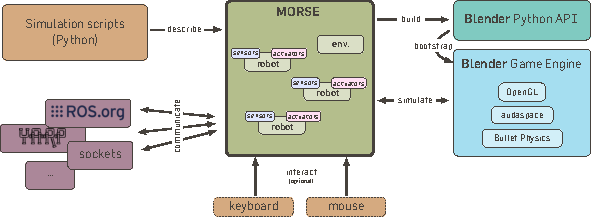
\includegraphics[width=\linewidth]{morse}
    \end{figure}
    \note {
        Describe the normal usage flow: Builder script $\rightarrow$
        MORSE build the scene using Blender API, then start the BGE
        $\rightarrow$ further interactions via middlewares.

        Humans \textbf{are robots}. We can \emph{optionally} use keyboard +
        mouse to control them.
    }

\end{frame}

\begin{frame}[fragile]
    \begin{multicols}{2}
    \null \vfill
    
    \begin{overprint}
    
    \onslide<1>
    \begin{minted}[fontsize=\scriptsize]{sh}
    > morse create my_sim

    > cd my_sim
    > ls
    default.py  scripts/  src/

    \end{minted}
    
    \onslide<2>
    \begin{minted}[fontsize=\scriptsize]{sh}
    > morse create my_sim

    > cd my_sim
    > ls
    default.py  scripts/  src/

    > morse run my_sim

    \end{minted}
    
    \onslide<3>
    \begin{minted}[fontsize=\scriptsize]{sh}
    > morse create my_sim

    > cd my_sim
    > ls
    default.py  scripts/  src/

    > morse run my_sim

    > cat default.py
    \end{minted}

    \end{overprint}
    \vfill \null
    \columnbreak
    \null \vfill

    \begin{overprint}
    %TODO: I can not get the picture (and the shell code in first col) to
    % correctly vertically align. Works if the minted env below if
    % commented out...
    \includegraphics<2>[width=\linewidth]{morse_default}
    \onslide<3>
    \begin{minted}[fontsize=\scriptsize]{python}
    #! /usr/bin/env morseexec
    from morse.builder import *
    robot = Morsy()
    robot.translate(1.0, 0.0, 0.0)

    motion = MotionVW()
    robot.append(motion)

    keyboard = Keyboard()
    robot.append(keyboard)

    pose = Pose()
    robot.append(pose)

    robot.add_default_interface('socket')

    env = Environment('sandbox')
    env.set_camera_location([ 10.0, 
                             -10.0, 
                              10.0])
    env.set_camera_rotation([1.05, 
                                0, 
                             0.78])
    \end{minted}
    \end{overprint}
    \vfill \null
    \end{multicols}

    \note{
        How is it like to actually use MORSE?

        Briefly explain default.py (illustrate the fact that
        robots are build out of actuators and sensors, and connected
        to one or several middlewares).
    }
    
\end{frame}


\begin{frame}{Levels of abstraction}
    \begin{figure}
        \centering
        \includegraphics<1>[width=\linewidth]{realism-0}
        \includegraphics<2>[width=\linewidth]{realism-1}
        \includegraphics<3>[width=\linewidth]{realism-2}
        \includegraphics<4>[width=\linewidth]{realism-3}
    \end{figure}
    \note{
        One of the strenghts of MORSE: the concept of 'abstraction level'.

        \begin{itemize}
            \item Fig1: MORSE only simulates the environment + cameras,
                remaining is done with the robot software stack
            \item Fig2: MORSE provides a depth image: no stereovision required
            \item Fig3: MORSE provides a terrain model: no reconstruction needed
            \item Fig4: semantic camera: MORSE provides the list of visible abstract
                objects.
        \end{itemize}
    }
    \end{frame}


\begin{frame}[fragile]
    \begin{multicols}{2}
        \null \vfill
\begin{pythoncode}
    from random import uniform
    from morse.builder import *

    robot = PR2()

    for h in range(30):
        human = Human()
        human.translate(
                uniform(-5, 5), 
                uniform(-5, 5), 
                0)

        human.rotate(
                0, 
                0, 
                uniform(0, 360))

    env = Environment('sandbox')
\end{pythoncode}

        \vfill \null
        \columnbreak
        \null \vfill
        \begin{figure}
            \centering
            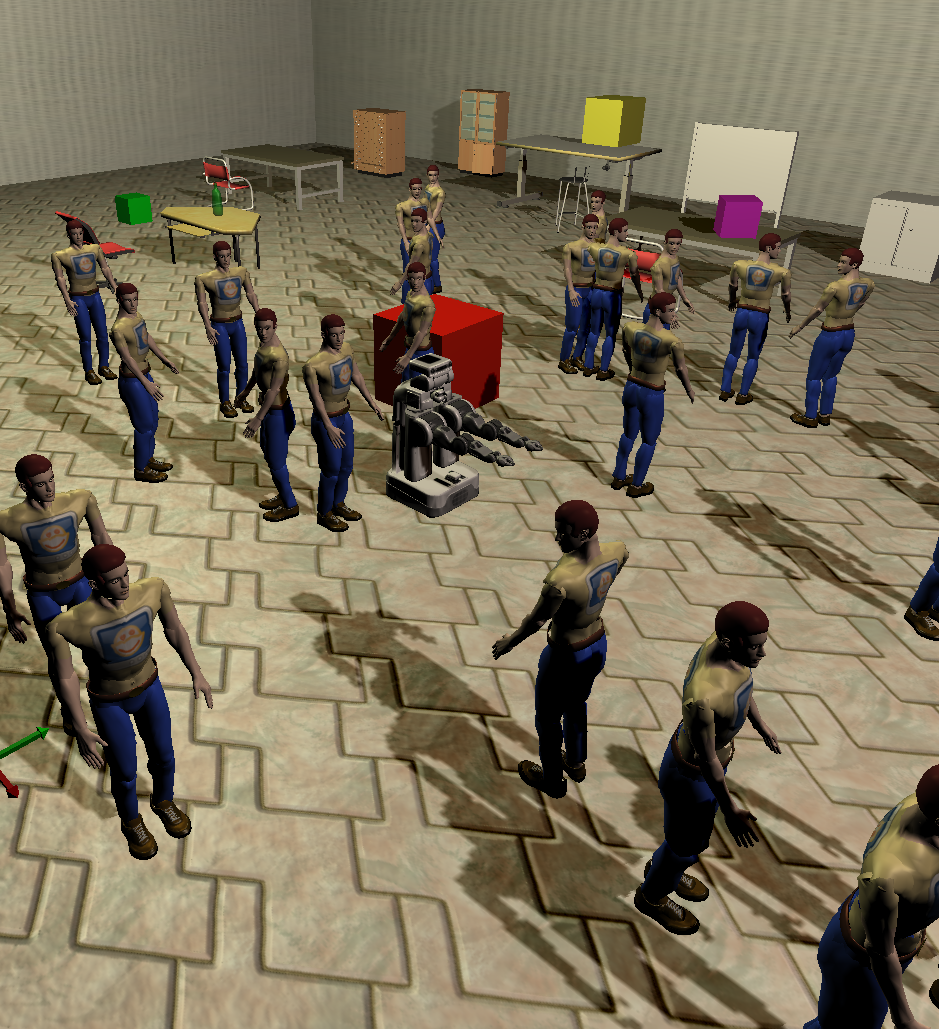
\includegraphics[width=\linewidth]{30humans}
        \end{figure}
        \vfill \null
    \end{multicols}

    \note{
        Describe how MORSE can easily be programmed to generate complex scenes.

        Note that in this example, humans won't move by themselves. For that,
        one need to add a motion actuator, and write and external script to
        control the crowd.
    }
\end{frame}

\imageframe[Not there yet...]{morse-hri}


%%%%%%%%%%%%%%%%%%%%%%%%%%%%%%%%%%%%%%%%%%%%%%%%%%%%%%%%%%%%%%%%%%%%%%%%%%%%
%%%%%%%%%%%%%%%%%%%%%%%%%%%%%%%%%%%%%%%%%%%%%%%%%%%%%%%%%%%%%%%%%%%%%%%%%%%%
%%%%%%%%%%%%%%%%%%%%%%%%%%%%%%%%%%%%%%%%%%%%%%%%%%%%%%%%%%%%%%%%%%%%%%%%%%%%

\section{Simulating HRI}

\begin{frame}{Situation Assessment with Human}
    \begin{figure}
        \centering
        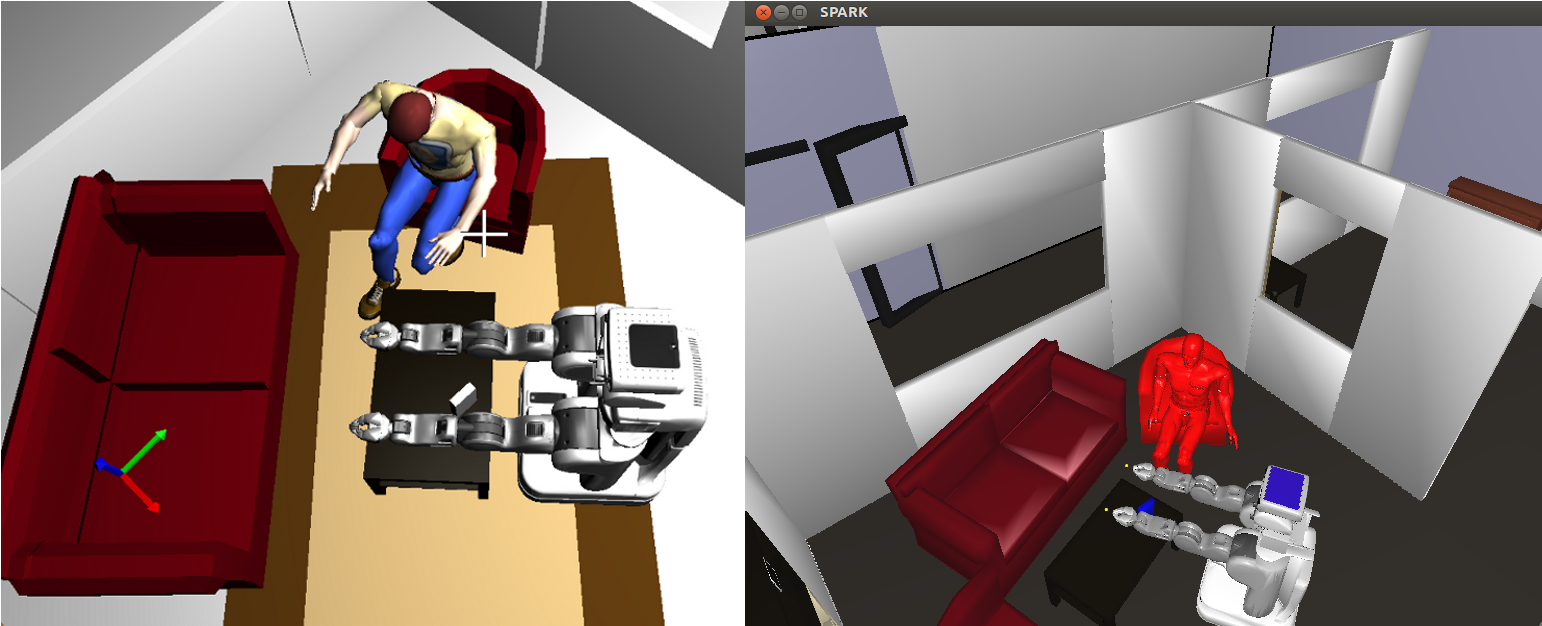
\includegraphics[width=\linewidth]{morsespark}
    \end{figure}
    \note {
        MORSE provides a virtual environment that we use to harness situation
        assessment algorithms that also include human-centered \emph{perspective
        taking}. The robot updates its knowledge using its own position, human
        position and objects seen through abstracted, symbolic cameras provided
        by MORSE (so-called \emph{semantic} cameras). In this particular
        scenario the human is sitting in a couch and ask the robot to bring
        specific objects that may be in another room (Pick-Place-Carry task).

    }
\end{frame}

\begin{frame}{Large Scenarii}
    \begin{figure}
        \centering
        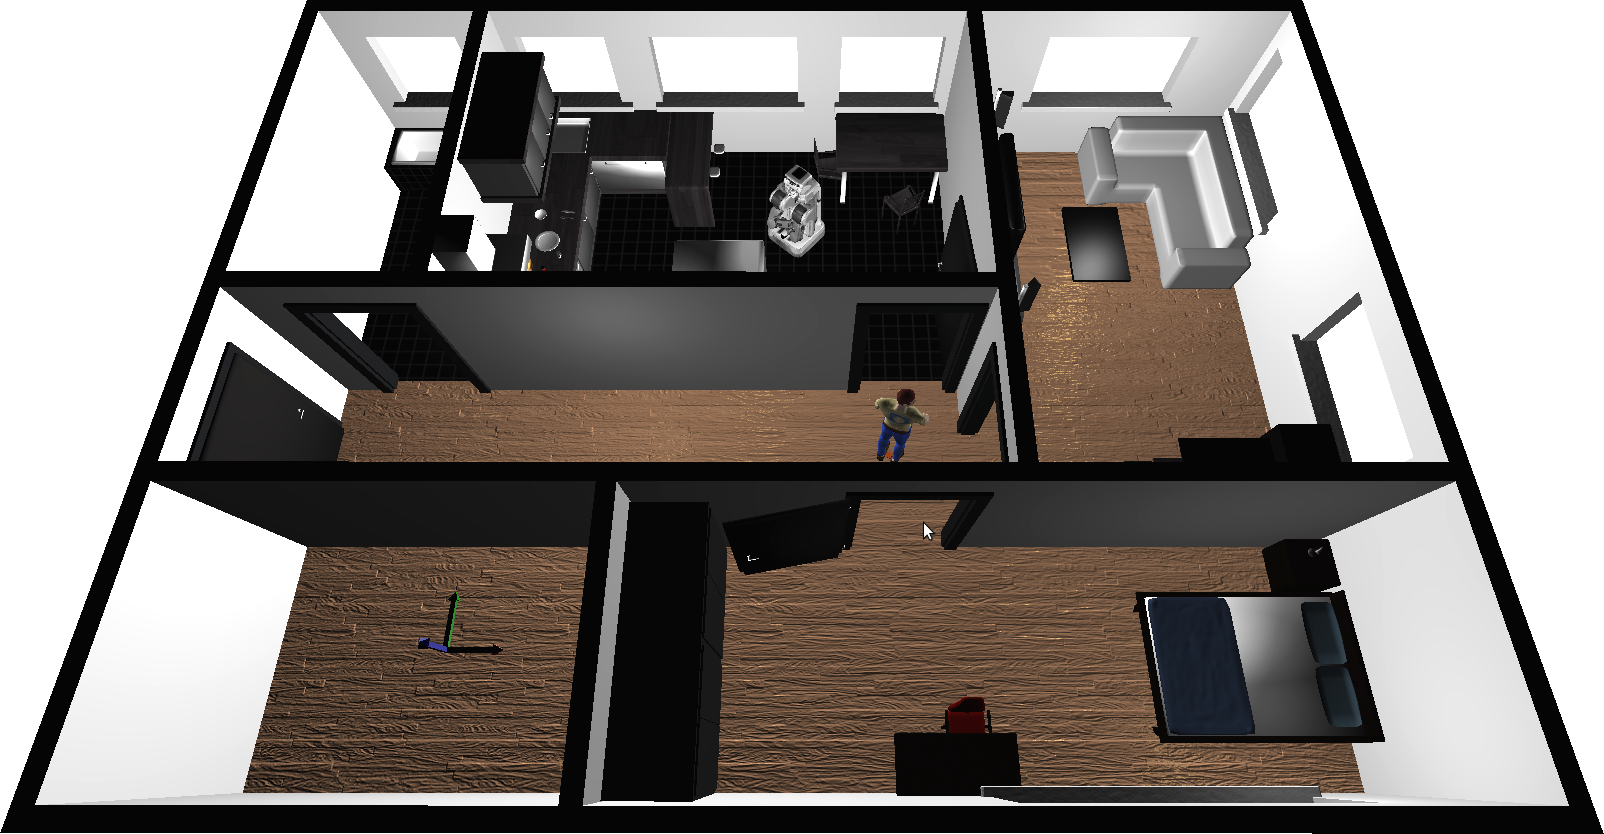
\includegraphics[width=\linewidth]{morse_apartment}
    \end{figure}
    \note {

        An apartment is simulated in which a domestic service robot is living
        together with a person.  A PR2 robot is controlled via ROS and the {\sc
        Cram} reactive plan language, which is used on several other real
        robots. The robots' duty is to observe the person performing different
        activities and detect unexpected situations based on the validation of
        different types of expectations.  The detection of such unexpected
        behavior can help future domestic service robots to better assess
        situations and adapt their actions to human behavior.

    }
\end{frame}

\begin{frame}{Refining Algorithms}
    \begin{multicols}{2}
        \null \vfill
    \begin{figure}
        \centering
        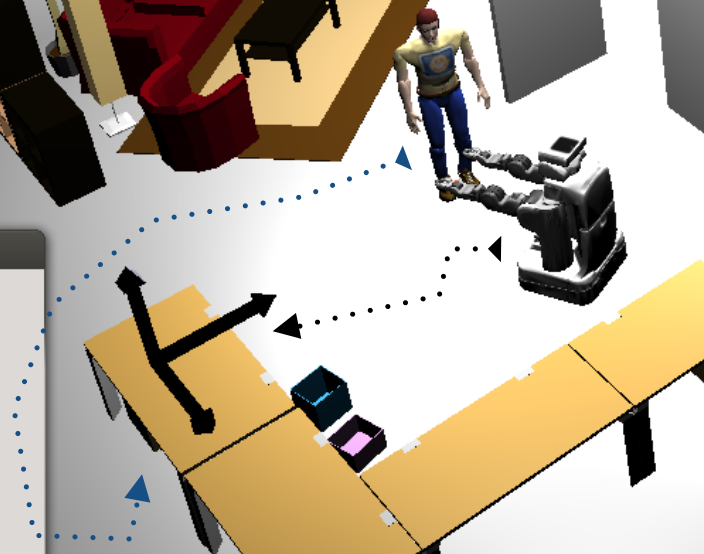
\includegraphics[width=0.9\linewidth]{proto-setup}
    \end{figure}

        \vfill \null
        \columnbreak
        \null \vfill
        \begin{figure}
            \centering
            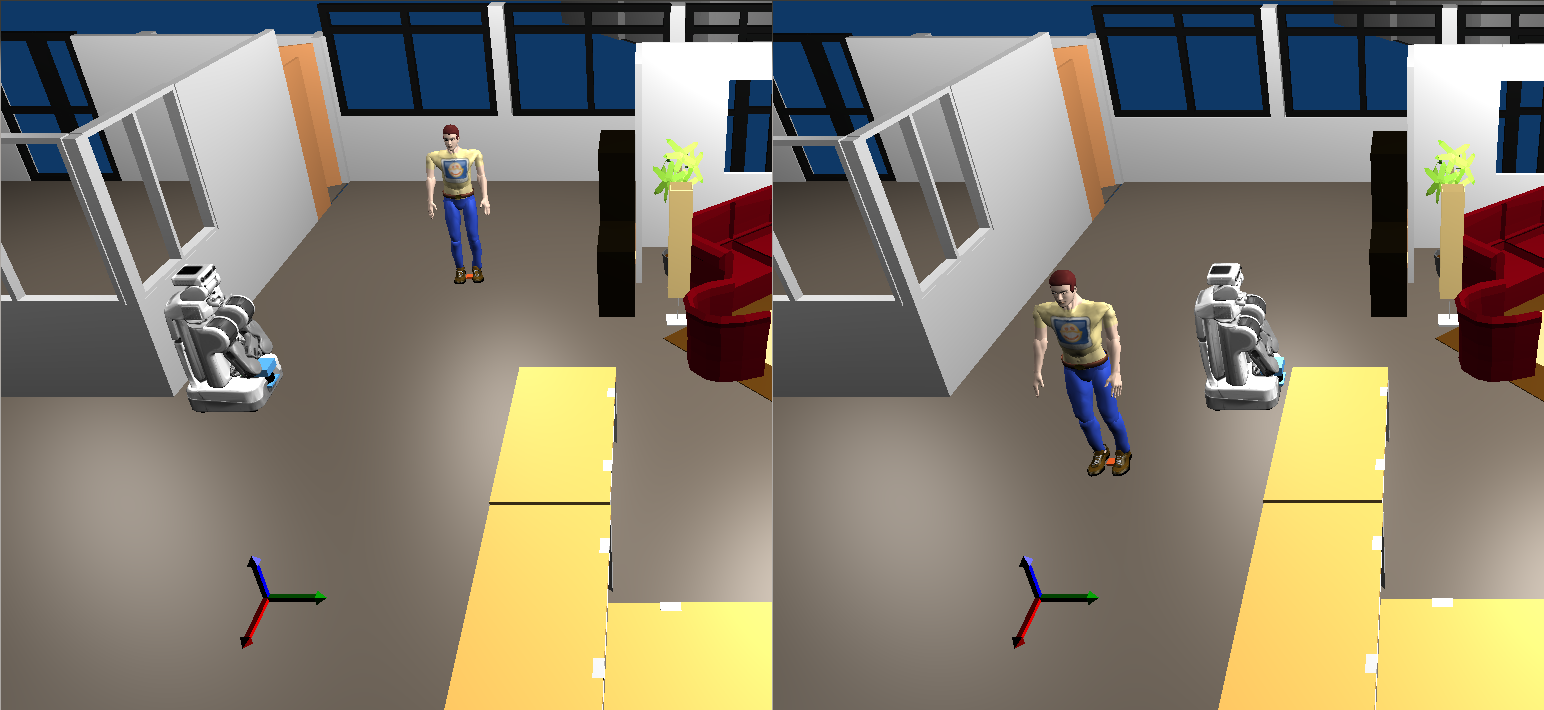
\includegraphics[width=0.9\linewidth]{morsehanp}
        \end{figure}
        \vfill \null
    \end{multicols}
    \note {
        Testing path planning algorithms (without killing humans and destroying
        robots...)
    }
\end{frame}

\begin{frame}{Benefits}
    \begin{itemize}
        \item Repeatable: fine for benchmarks, regression tests,
        \item Abstraction levels: simulate only what is needed,
        \item \emph{Computer game}-style, tests can be carried by one researcher
            alone: support iterative design and implementation,

    \end{itemize}
\end{frame}


\section{Less Usual Use-cases}

\begin{frame}{Automatic Human-like Scene Generation}
    \begin{figure}
        \centering
        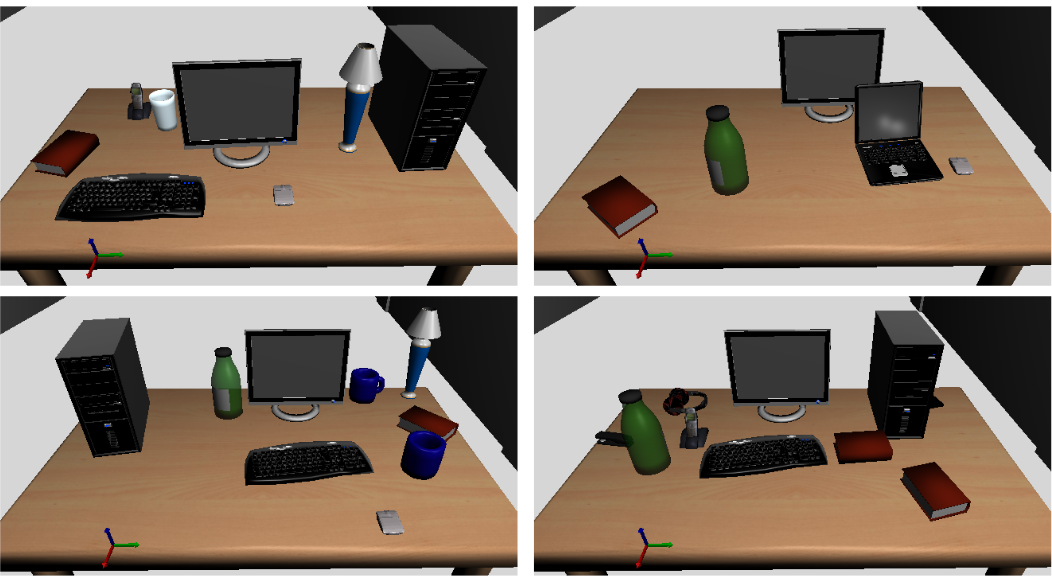
\includegraphics[width=\linewidth]{scenes}
    \end{figure}
    \note {
        Aim: simulating credible human environments to train systems to appropriately
react to them.

Robots need to know, when, where and how people manipulate objects and how they
arrange and structure them in space $\rightarrow$ understand the long-term,
spatio-temporal relationships of objects and activities of people.

We look at learning qualitative spatial relations of objects on office desks.
As an accurate classification and pose estimation of objects on real-world
office desks is still a challenging and difficult task for current robot
perception systems we acquired a data set of object arrangements using the MORSE
simulator. For this, we automatically generated a set
of physically possible desktop scenes. Based on the generated data we
learned relational models of object arrangements on desks. The learnt models
enabled a robot to predict the position of an object given a landmark.


    }
\end{frame}


\begin{frame}{Continuous Integration and HRI}
    \begin{figure}
        \centering
        %\includegraphics[width=\linewidth]{}
    \end{figure}

    \note {
        In human-robot interaction studies, robots often indicate behavioral
        variability that may influence the experiment's final outcome.  However,
        manual testing on physical systems is usually the only way to prevent
        this, but remains labour-intensive. To tackle this issue, we introduced
        \emph{early automated prototype testing}.

        The goal is to incrementally decrease the level of abstraction until a
        satisfactory/sufficient degree of ``realism'' to make an assumption
        about real world behavior is reached --- in an integrated and continuous
        approach.

    }
\end{frame}


\section{What Next?}

\imageframe[Soon there?]{morse-hri}

\begin{frame}{MakeHuman Integration}
    \begin{figure}
        \centering
        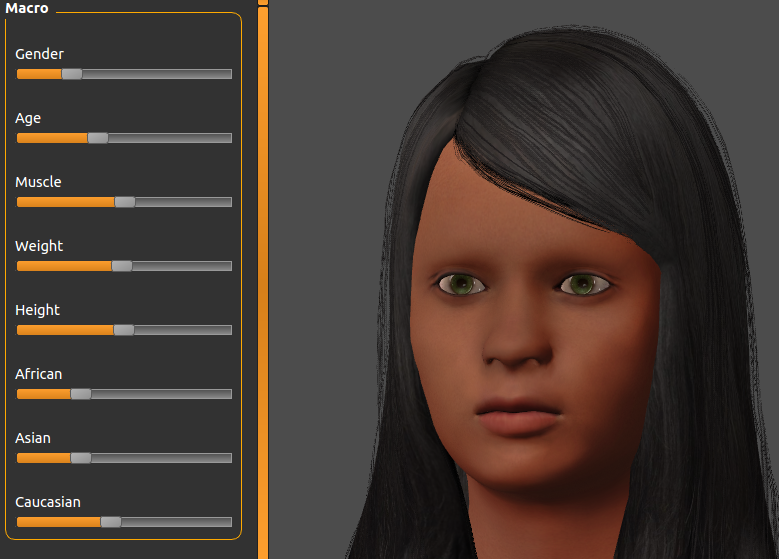
\includegraphics[width=\linewidth]{makehuman}
    \end{figure}
    \note{
        More realistic human models, possibly procedurally generated.
    }
\end{frame}


\begin{frame}{What Next?}
    \begin{itemize}
        \item<1-> Autonomous navigation of humans
        \item<2-> Crowd simulation
        \item<3-> Better library of motions (walk cycles, pick/place, emotions...)
    \end{itemize}

    \uncover<4->{
    Open "HRI" issues on GitHub: \url{https://github.com/morse-simulator/morse/labels/HRI}
}
\end{frame}


\begin{frame}

    Thank you!

    \url{http://morse-simulator.github.io/}
\end{frame}
\end{document}






